\documentclass{report}
\usepackage[utf8]{inputenc}
\setcounter{tocdepth}{5}
\setcounter{secnumdepth}{5}
\renewcommand{\contentsname}{Indice}


\title{
    MoMa \\
    \large Applicazioni e Servizi Web
}

\author{Michele Torroni - 0001050680 \{michele.torroni@studio.unibo.it\}}
\date{23 Giugno 2022}



\usepackage{natbib}
\usepackage{graphicx}
\usepackage{setspace}
\usepackage{subfigure}
\usepackage{float}
\usepackage{listings}
\usepackage{hyperref}
\doublespacing

\begin{document}
\maketitle
\tableofcontents
\newpage
\linespread{1.2}


\section{Introduzione}
MoMa (abbreviazione di “Money Manager”) é un’applicazione web che consente agli utenti di tenere traccia delle proprie transazioni monetarie.
\newline
\newline
Il sistema fornisce la possibilità di creare categorie di spesa (“categories”, ad esempio: “food”, “shopping”, “presents”) e dei portafogli (“wallets”, ad esempio: “wallet”, “credit card”) al fine di categorizzare le transazioni; infatti ogni spesa é discriminata da una category e un wallet di riferimento, e, alla creazione, MoMa aggiorna in automatico i dati di tutte le entità in gioco, in modo da fornire all’utente uno storico quanto piú preciso possibile.
\newline
\newline
Per fornire un’adeguata sicurezza dei contenuti, il sistema richiede un’iscrizione (con password) e l’utente potrà decidere in qualsiasi momento di eliminare tutti i contenuti (compreso il proprio account) dall’applicazione.
\newpage

\section{Requisiti}
\subsection{Requisiti Funzionali}
L’utente all’interno dell’applicazione potrà:
\begin{itemize}
    \item   Creare il proprio profilo, consistente in uno username, una password e un’immagine;
    \item	Modificare tutte le informazioni del proprio account dopo aver effettuato l’accesso, compresa la possibilità di cancellare il profilo e tutti i dati ad esso collegati;
    \item	Creare le proprie categorie di spesa, ognuna con un nome e un colore di riferimento;
    \item	Modificare e cancellare le categorie create e le transazioni ad esse collegate;
    \item	Creare i propri portafogli, con un nome e un colore ciascuno, analogamente a quanto accade per le categorie, oltre ad un saldo di partenza;
    \item	Aggiornare il saldo dei portafogli;
    \item	Eliminare i portafogli e tutte le transazioni ad essi collegate;
    \item	Creare transazioni, discriminate da una categoria e un portafoglio di riferimento, oltre ad un nome, un ammontare in denaro e una data;
    \item	Eliminare le transazioni;
    \item	Filtrare le transazioni per intervallo di date, categoria e portafoglio di riferimento;
\end{itemize}
\newpage

\subsection{Requisiti Non Funzionali}
L’applicazione dovrà:
\begin{itemize}
    \item 	Avere un’interfaccia responsiva;
    \item 	Essere Accessibile, semplice e facilmente interpretabile;
    \item 	Fornire meccanismi di autenticazione sicuri;
    \item 	Essere estensibile con nuove funzionalità;
\end{itemize}

\subsection{Requisiti Di Implementazione}
L’applicazione dovrà:
\begin{itemize}
    \item Essere sviluppata utilizzando lo stack M.E.V.N.;
    \item Utilizzare MongoDB come DBMS (non relazionale);
    \item Fare utilizzo della libreria Socket.IO per fornire comunicazioni real-time;
\end{itemize}

\newpage

\section{Design e Architettura}
\subsection{Design}
L’applicazione é stata sviluppata facendo uso dello stack MEVN, una variante dello stack MEAN (in cui viene utilizzato il framework javascript Vue.Js in sostituzione ad Angular.Js) e il cui acronimo rappresenta le tecnologia utilizzate:
\begin{itemize}
    \item 	MongoDB
    \item 	Express
    \item	React
    \item 	Node.js
\end{itemize}
Queste tecnologie verranno descritte nello specifico all’interno del capitolo 4.
\newline \newline
Durante lo svolgimento del progetto si é fatto fede ai principi KISS (“Keep It Stupid, Simple”) e DRY (“Don’t Repeat Yourself”), notevolmente aggevolati dal meccanismo dei “components” fornito da Vue.Js.
\newline \newline
Il Design dell’applicativo si basa sul modello iterativo UCD (acronimo di “User Centered Design”), con utenti virtualizzati mediante il meccanismo delle “Personas”: si tratta di utenti target “immaginari”, ma con caratteristiche peculiari riscontrabili in individui reali.

\subsection{Architettura Sistema}
L’architettura del sistema é ascrivibile al modello REST (“Representational State Transfer”), nella quale le comunicazioni
avvengono su HTTP e il sistema é di tipo “stateless”.
\newline \newline
L’applicazione puó essere descritta mediante quattro Entità:
\begin{enumerate}
    \item User: utente finale che utilizza il sistema e ha la completa proprietà dei propri dati;
    \item Categories: categorie di spesa, personalizzabile nel colore e nel nome, che deve essere univoco all’interno delle categorie dell’utente;
    \item Wallets: portafogli, che modellano tutti i possibili loci in cui l’utente conserva i propri risparmi, come “salvadanaio”, “conto corrente”, “carta prepagata”, ecc…;
    \item Transactions: transazioni, che rappresentano le spese dell’utente, ognuna delle quali si riferisce ad una specifica categoria e uno specifico portafoglio.
\end{enumerate}
Di seguito uno schema riassuntivo delle relazioni tra le entità.
\begin{figure}[H]
    \centering
    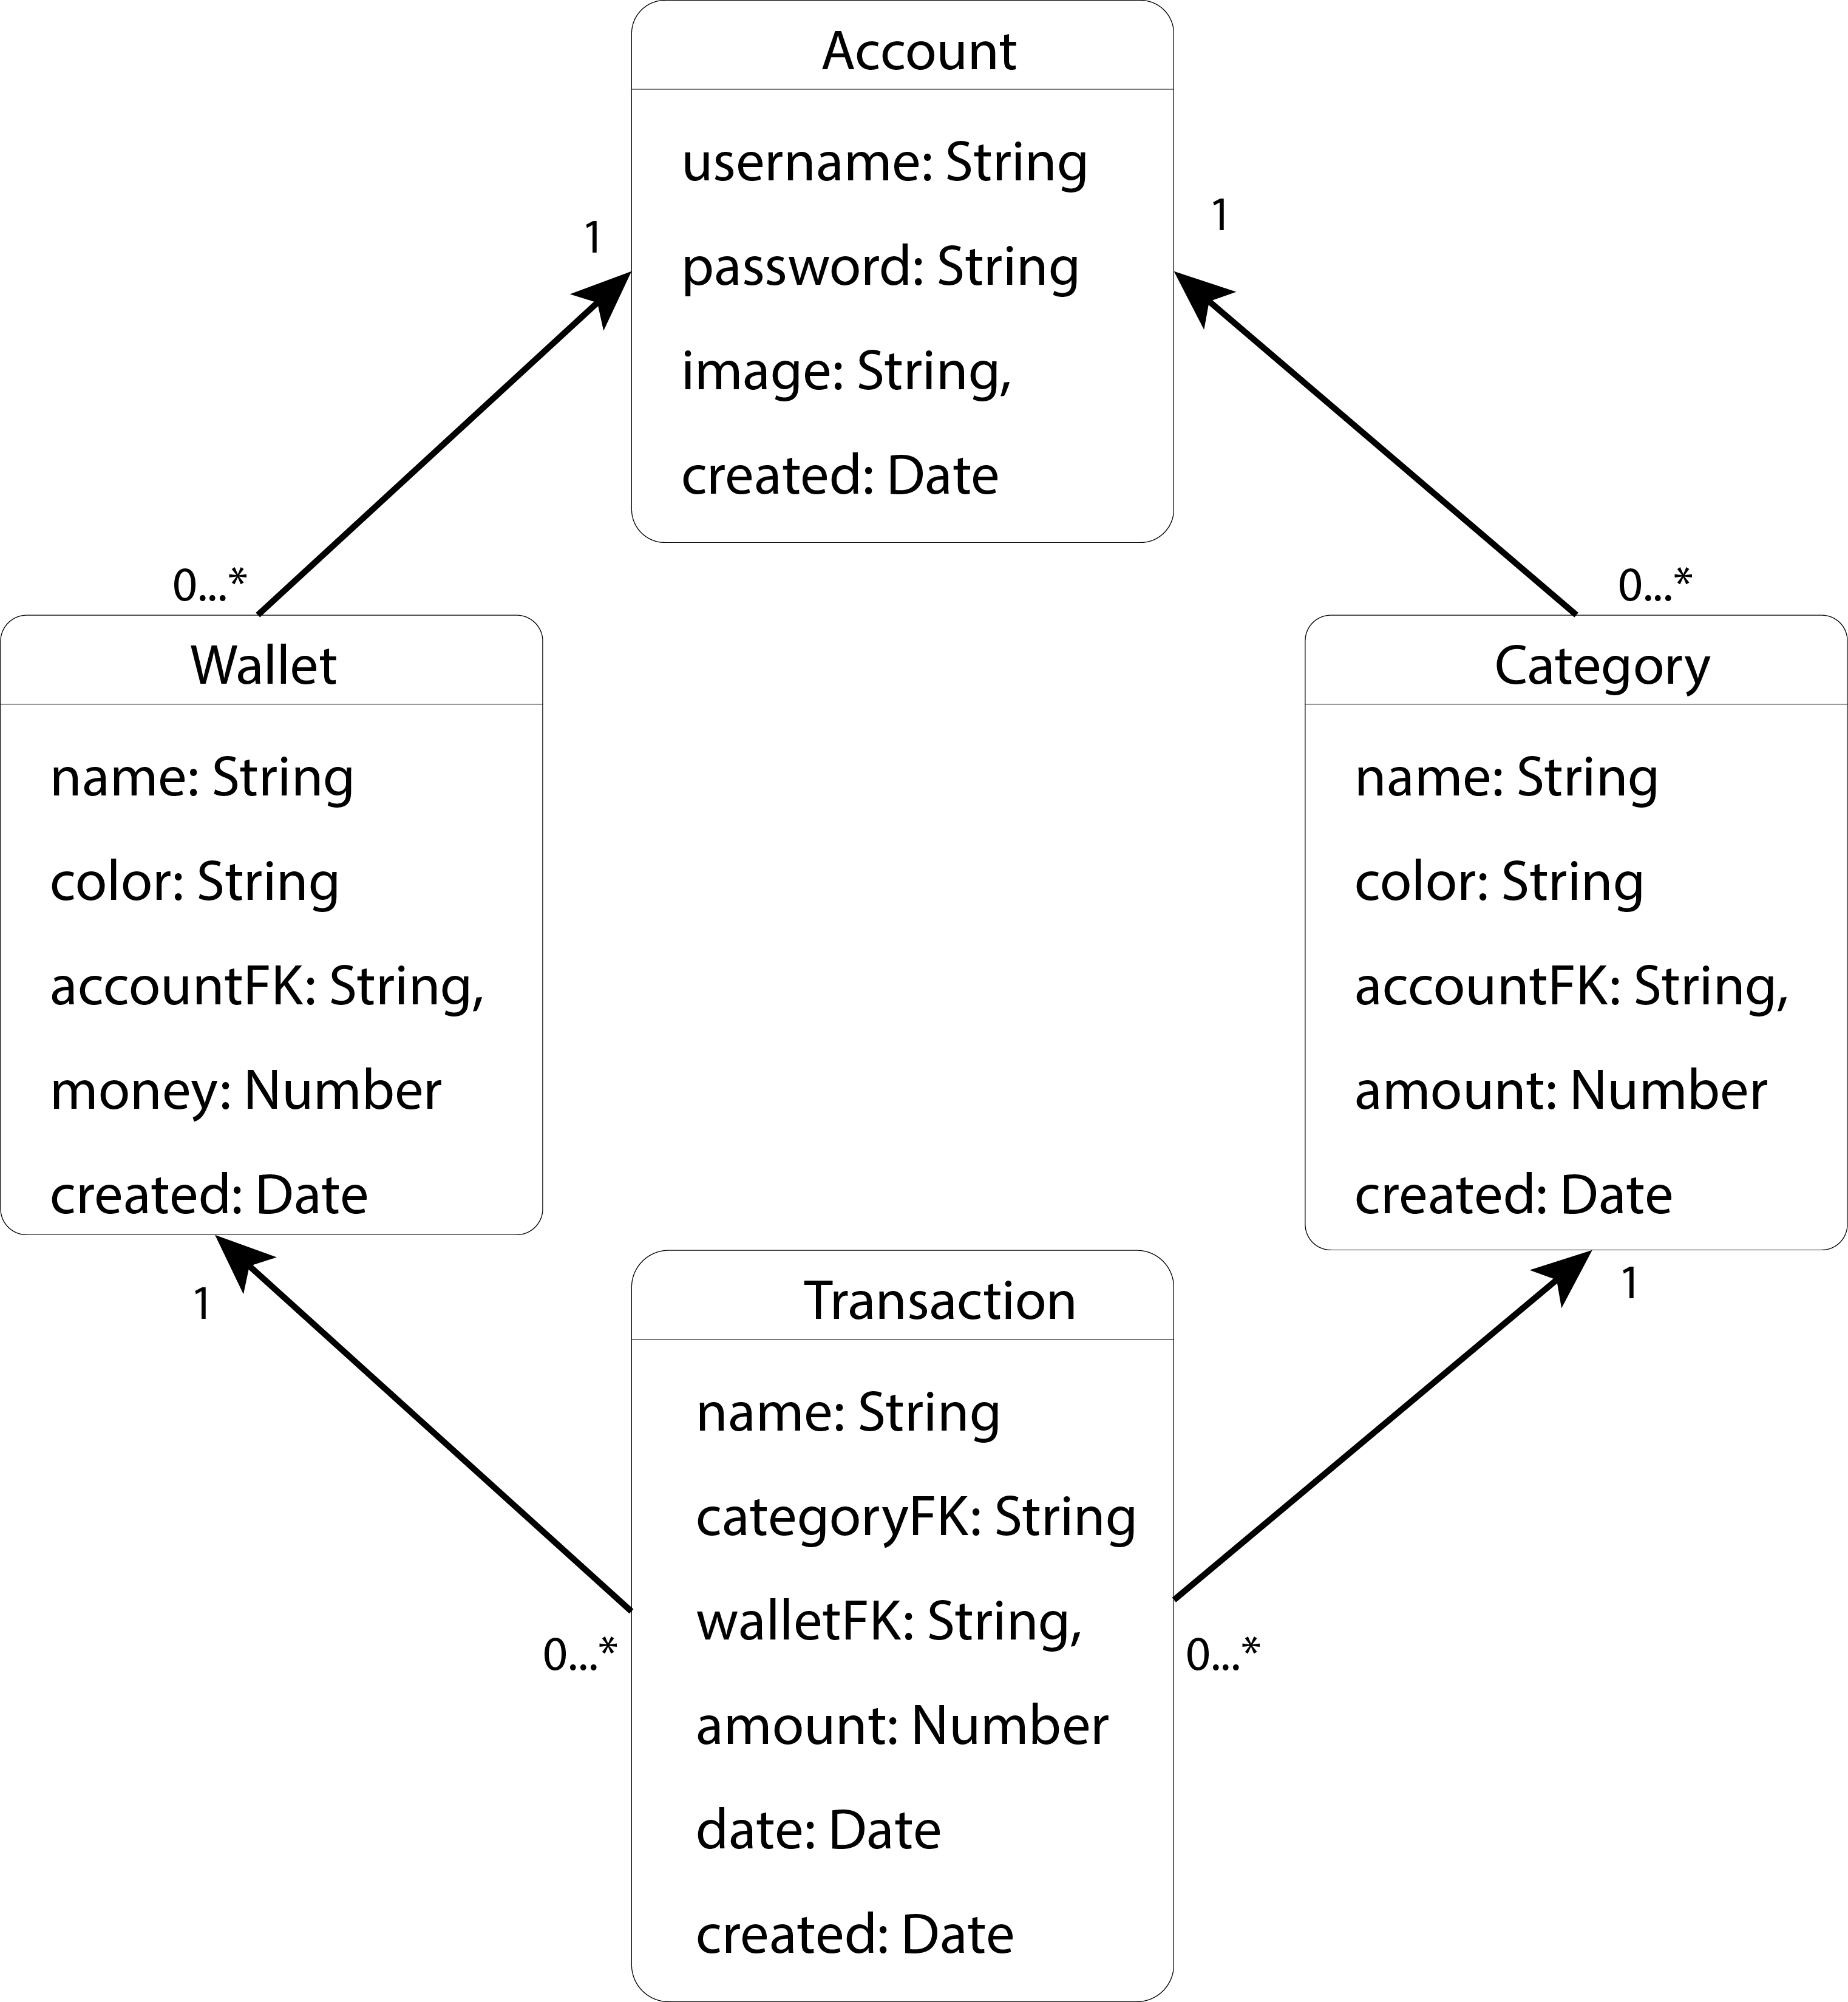
\includegraphics[scale=0.08]{images/UML.png}
    \caption{Schema Entità e relazioni}
\end{figure}

N.B. tutte le entità in gioco sono collegate al solo utente proprietario di quelle informazioni, per garantire il “Diritto all’oblio” dell’utente nel caso in cui esso sia intenzionato ad eliminare il proprio account e tutte le informazioni ad esso collegate.

\subsection{Architettura Interfacce Utente – Mockup e StoryBoard}
Di seguito si presentano i mockups disegnati in fase di analisi del progetto a confronto con le corrispondenti schermate sviluppate, in quanto queste ultime seguono quasi fedelmente le idee dei bozzetti.

\subsubsection{Login}
Appena l’utente apre l’applicazione web si trova davanti alla schermata di login, in cui deve inserire username e password con cui ha eseguito l’iscrizione al sistema.
\begin{figure}[H]
    \begin{subfigure}
        \centering
        \includegraphics[scale=0.3]{images/mockups/Login.png}
        \caption{Mockup Login}
    \end{subfigure}
    \par\bigskip
    \begin{subfigure}
        \centering
        \includegraphics[scale=0.35]{images/screens/Login.png}
        \caption{Screen Login}
    \end{subfigure}
\end{figure}

\subsubsection{Sign Up}
Se l’utente non ha ancora effettuato il Sign Up all’applicazione, potrà registrarsi mediante l’apposita schermata, accessibile da un link posizionato in basso a sinistra della schermata di Log In.
\newline
La schermata presenta la possibilità di inserire un’immagine di profilo, uno username e una password (che deve essere ripetuta correttamente al fine di procedere all’iscrizione al sistema).
\newline
L’interfaccia presenta eventuali errori all’utente (come “username already used”) mediante un banner posizionato sotto ai campi compilabili
\begin{figure}[H]
    \begin{subfigure}
        \centering
        \includegraphics[scale=0.3]{images/mockups/Sign Up.png}
        \caption{Mockup Sign Up}
    \end{subfigure}
    \par\bigskip
    \begin{subfigure}
        \centering
        \includegraphics[scale=0.35]{images/screens/Sign Up.png}
        \caption{Screen Sign Up}
    \end{subfigure}
\end{figure}

\subsubsection{Application Layout}
Succesivamente ad aver effettuato l’accesso, l’utente potrà interagire con l’applicazione, che presenta una struttura composta da tre componenti:
\begin{enumerate}
    \item Una Toolbar, contente un icona “menu a panino”, il nome dell’applicazione, lo username dell’utente connesso e la sua immagine di profilo
    \item Una Sidebar apribile/nascondibile con il sopracitato menu a panino, e che contiene i link di navigazione alle varie schermate dell’applicazione
    \item Tutta la porzione rimanente dell’interfaccia contiene le informazioni contestuali alla schermata navigata (verranno presentati ai punti 3.3.6.x di questa tesi di progetto)
\end{enumerate}
In aggiunta, tutte le schermate accessibili mediante la sidebar presentano un “floating button” in basso a destra che permette di creare una nuova entità, contestualmente alla schermata in cui ci si trova (es: Categories -> Add Category)
\begin{figure}[H]
    \begin{subfigure}
        \centering
        \includegraphics[scale=0.3]{images/mockups/Application.png}
        \caption{Mockup Application Layout}
    \end{subfigure}
    \par\bigskip
    \begin{subfigure}
        \centering
        \includegraphics[scale=0.35]{images/screens/Application.png}
        \caption{Screen Application Layout}
    \end{subfigure}
\end{figure}


\paragraph{Categorie}
\subparagraph{Categories}
Schermata che mostra le categorie dell’utente, mediante card colorate (colore selezionabile dall’utente) disposte con un layout a “griglia adattiva”.
\begin{figure}[H]
    \begin{subfigure}
        \centering
        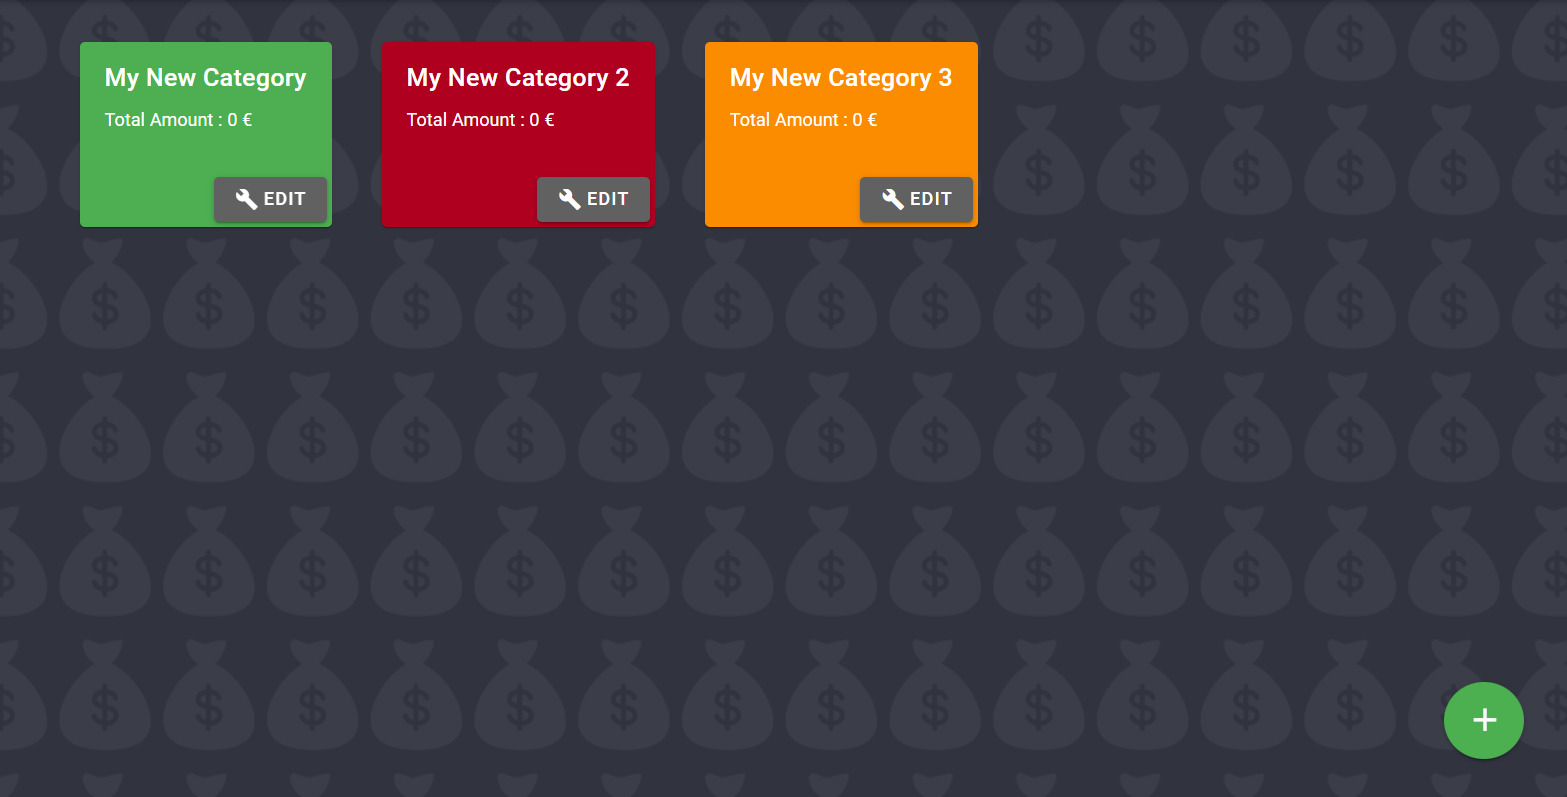
\includegraphics[scale=0.3]{images/mockups/Categories.png}
        \caption{Mockup Categories}
    \end{subfigure}
    \par\bigskip
    \begin{subfigure}
        \centering
        \includegraphics[scale=0.35]{images/screens/Application.png}
        \caption{Screen Categories}
    \end{subfigure}
\end{figure}


\subparagraph{Add Category}
Schermata, accessibile mediante il floating button citato a 3.3.6, che permette di aggiungere una nuova categoria
\begin{figure}[H]
    \begin{subfigure}
        \centering
        \includegraphics[scale=0.3]{images/mockups/Add Category.png}
        \caption{Mockup Add Category}
    \end{subfigure}
    \par\bigskip
    \begin{subfigure}
        \centering
        \includegraphics[scale=0.35]{images/screens/Add Category.png}
        \caption{Screen Add Category}
    \end{subfigure}
\end{figure}

\subparagraph{Edit Category}
Al click sul pulsante “Edit” (presente sulla card delle Categorie), verrà aperta la schermata di editing della categoria selezionata, dove sarà inoltre possibile eliminare l’entità.
\begin{figure}[H]
    \begin{subfigure}
        \centering
        \includegraphics[scale=0.3]{images/mockups/Edit Category.png}
        \caption{Mockup Edit Category}
    \end{subfigure}
    \par\bigskip
    \begin{subfigure}
        \centering
        \includegraphics[scale=0.35]{images/screens/Edit Category.png}
        \caption{Screen Edit Category}
    \end{subfigure}
\end{figure}

\paragraph{Portafogli}
\subparagraph{Wallets}
Schermata di visualizzazione dei portafogli, accessibile mediante apposito link nella sidebar. I Wallets sono presentati mediante card “orizzontali”, attraverso le quali é possibile eliminare il portafoglio (e le relative transazioni), oltre a poter aggiungere e togliere denaro.
\begin{figure}[H]
    \begin{subfigure}
        \centering
        \includegraphics[scale=0.3]{images/mockups/Wallets.png}
        \caption{Mockup Wallets}
    \end{subfigure}
    \par\bigskip
    \begin{subfigure}
        \centering
        \includegraphics[scale=0.35]{images/screens/Wallets.png}
        \caption{Screen Wallets}
    \end{subfigure}
\end{figure}

\subparagraph{Add Wallet}
Schermata, accessibile mediante il floating button citato a 3.3.6, che permette di aggiungere un nuovo portafoglio.
\begin{figure}[H]
    \begin{subfigure}
        \centering
        \includegraphics[scale=0.3]{images/mockups/Add Wallet.png}
        \caption{Mockup Add Wallet}
    \end{subfigure}
    \par\bigskip
    \begin{subfigure}
        \centering
        \includegraphics[scale=0.35]{images/screens/Add Wallet.png}
        \caption{Screen Add Wallet}
    \end{subfigure}
\end{figure}

\paragraph{Transazioni}
\subparagraph{Transactions}
Schermata di visualizzazione delle transazioni, accessibile mediante apposito link nella sidebar oppure cliccando su una card dei Wallets o delle Categories e, in questi casi, la pagina si apre con i filtri prevalorizzati con l’elemento scelto. Le Transactions si presentano come card “orizzontali”, attraverso le quali é possibile eliminare la transazione.
\begin{figure}[H]
    \begin{subfigure}
        \centering
        \includegraphics[scale=0.3]{images/mockups/Transactions.png}
        \caption{Mockup Transactions}
    \end{subfigure}
    \par\bigskip
    \begin{subfigure}
        \centering
        \includegraphics[scale=0.35]{images/screens/Transactions.png}
        \caption{Screen Transactions}
    \end{subfigure}
\end{figure}

\subparagraph{Add Transaction}
Schermata, accessibile mediante il floating button citato a 3.3.6, che permette di aggiungere una nuova transazione. Sono presenti due dropdown, relative rispettivamente ai Wallets e alle Categories, grazie alle quali é possibile scegliere gli estremi della transazione.
\begin{figure}[H]
    \begin{subfigure}
        \centering
        \includegraphics[scale=0.3]{images/mockups/Add Transaction.png}
        \caption{Mockup Add Transaction}
    \end{subfigure}
    \par\bigskip
    \begin{subfigure}
        \centering
        \includegraphics[scale=0.35]{images/screens/Add Transaction.png}
        \caption{Screen Add Transaction}
    \end{subfigure}
\end{figure}

\paragraph{Account}
Schermata relativa alle informazioni dell’utente, raggiungibile dal relativo link all’interno della sidebar oppure cliccando l’immagine dell’utente nella toolbar in cima alla pagina. É possibile modificare tutte le informazioni dell’utente (Username, Immagine e Password) oppure eliminare il profilo, ma é necessario inserire la password precedentemente inserita (come prevenzione).
\begin{figure}[H]
    \begin{subfigure}
        \centering
        \includegraphics[scale=0.3]{images/mockups/Account Settings.png}
        \caption{Mockup Account Settings}
    \end{subfigure}
    \par\bigskip
    \begin{subfigure}
        \centering
        \includegraphics[scale=0.35]{images/screens/Account Settings.png}
        \caption{Screen Account Settings}
    \end{subfigure}
\end{figure}

\subsection{Design di dettaglio}
\subsubsection{Backend}
Il backend é stato sviluppato attraverso l’uso delle tecnologie Express, Mongoose e Socket.Io.
\newline
I controllers sono rappresentati da classi javascript che espongono API per interagire con il backend, nello specifico sono presenti operazioni di tipo CRUD (Create, Read, Update, Delete) e sfruttano I Models, ovvero classi javascript che esportano Mongoose Schemas (rappresentazioni della struttura delle entità). Nel progetto si é mantenuta ove possibile una struttura “1 a 1” per ogni entità, quindi sono presenti quattro file di controller,  quattro di model e quattro di routes.
\newline
I file di routes utilizzano Express per fornire path e metodi specifici per richiamare le web Api esposte dai controller.
\newline
L’entry point del backend (“./server” nei file di progetto) é il file “app.js”, che fa uso di Express, Mongoose, Socket.Io e dei file di route sopracitati. Socket.Io é utilizzato all’interno del progetto per rendere possibile la sincronizzazione in tempo reale delle operazioni effettuate dal medesimo utente su piú dispositivi/istanze dell’applicazione.
\newline
Le immagini utente vengono salvate all’interno del backend (nella directory ‘./uploads’ statica) grazie alla libreria node “Multer”.

\subsubsection{Frontend}
Il frontend é stato sviluppato utilizzando il framework javascript Vue.Js 3.0, Vue-router e la libreria node Vuetify, che mette a disposizione componenti (discriminati dall’apposizione di  “v-” nel tag html) nativamente reattivi e in stile material design.
\newline \newline
La struttura dell progetto Frontend (“./client/src” nell’applicativo)  si compone di sei parti principali:
\begin{enumerate}
    \item Il file javascript “main.js”, entry point dell’applicazione e resposabile dell’instanziamento di Vue, Vuetify e router;
    \item Il file Vue “App.vue”, vero e propria root dell’instanza di Vue;
    \item Directory “views”, al cui interno risiedono tutte le schermate esposte ai punti 3.3.* e sviluppate come file Vue, in maniera quindi modulare;
    \item Directory “router”, contenente il file “index.js” responsabile del routing di Vue-router;
    \item Directory “components”, al cui interno sono presenti componenti riutilizzabili all’interno dell’applicazione, come floating button e message confirm, oltre ad un componente che gestisce le comunicazioni con socket.Io;
    \item Directory “Api”, al cui interno sono presenti, in maniera speculare al backend, i quattro file javascript responsabili delle chiamate alle api delle entità.
\end{enumerate}

\subsection{Tartget User Analysis}
Il target principale del sistema é un individuo che vuole tener traccia delle proprie spese e non gli basta o non puó o non vuole utilizzare le applicazioni bancarie.
\newline \newline
Di seguito vengono caratterizzate diverse personas, differenti per esigenze e modalità di utilizzo del sistema

\subsubsection{Personas: Giacomo}
Giacomo é un ragazzo minorenne che non ha ancora un conto bancario ma gli piacerebbe tener traccia delle sue spese (date le limitate finanze) ed essere sempre a conoscenza dell’ammontare di soldi che possiede tra portafoglio e salvadanaio e carta prepagata.
\newline \newline
Scenario d’uso: Giacomo riceve una paghetta di 50€ dai genitori e si compra un panino come merenda a scuola, per un totale di 2.50€.
\begin{itemize}
    \item Giacomo accede alla piattaforma;
    \item Si iscrive registrando i propri dati e inserendo la foto scattata poco prima con il suo cane;
    \item Crea subito una category “Merenda a scuola” e  un wallet “Portafoglio”.
    \item Aggiunge 50€ al portafoglio.
    \item Crea una transazione “Panino con la cotoletta”, con data odierna, valore di 2.50€, della categoria “Merenda a scuola” e wallet “Portafoglio”.
    \item Dalle relative schermate nota che per la categoria “Merenda a scuola” ha speso per ora un totale di 2.50€ e nel portafoglio gli rimangono 47.50 €.
\end{itemize}

\subsubsection{Personas: Francesca}
Francesca é un’imprenditrice di successo e possiede molti conti in banche separate (che non comunicano tra loro). Francesca vorrebbe una soluzione per segnare tutte le spese che esegue e tenere traccia del conto con piú spese.
\newline \newline
Scenario d’uso: Francesca vuole comprarsi una nuova auto sportiva, ma non si ricorda in quale conto ha abbastanza fondi al momento.
\begin{itemize}
    \item Francesca accede alla piattaforma;
    \item Disponendo già delle credenziali di accesso, inserisce i propri username e password;
    \item Crea una nuova categoria “Automobili”;
    \item Controlla tra I wallet quale ha abbastanza denaro per l’auto dei suoi sogni e nota che é il conto corrente “Banca Verde”;
    \item Inserisce una transazione in data odierna, del valore *****€, categoria “Automobili” e wallet “Banca Verde”
\end{itemize}

\newpage

\section{Tecnologie}
Il progetto, come sopra evidenziat, é stato sviluppato utilizzando il solution stack MEVN e le principali tecnologie utilizzate sono state:
\begin{itemize}
    \item MongoDB e Mongoose
    \item Express
    \item Vue.js, Vue Router e Vuetify
    \item Node.js
    \item Socket.IO
    \item Docker
\end{itemize}

\subsection{MongoDB e Mongoose}
Lato backend, per gestire la persistenza dei dati, si é fatto uso di MongoDB come DBMS non relazionale e Mongoose.
\newline \newline
MongoDB, anche grazie alla sua natura non relazionale, puó essere classificato come database di tipo NoSQL, molto piú permissivo in termine di struttura dei dati grazie all’utilizzo di documenti in stile JSON per la persistenza dei dati.
\newline \newline
Mongoose é una libreria (scaricabile dal package manager di Node.js, ovvero “npm”) orientata agli oggetti e in grado di creare una connessione tra il framework Express e il database MongoDB. Questa tecnologia mette a disposizione una funzione “Schema()” che produce oggetti su cui é possibile chiamare le classiche procedure di interffacciamento al db.

\subsection{Express}
Express é un server framework open source per applicazioni web sviluppate con Node.js, progettato per creare Web API e generare percorsi per le chiamate alle stesse.

\subsection{Vue.js, Vue Router e Vuetify}
Vue.js è un framework progressivo e monolitico JavaScript open-source per la creazione di interfacce utente e single-page applications in ambito web.
\newline
Con il termine single-page applications s’intende un’applicazione web che mette a disposizione utente una singola pagina, al fine di fornire un’esperienza simile ad un’applicazione desktop anche se si trova sul browser web. Questa soluzione è particolarmente performante dal punto di vista dell’utilizzatore poiché tutto il codice necessario (HTML, CSS, JavaScript, ecc…) è caricato all’apertura della pagina e, in risposta di azione dell’utente, vengono caricate e sostituite dinamicamente le risorse appropriate senza ricaricare la pagina web [Vue].
\newline
Vue.js è un framework in configurazione MVVM, ovvero Model-View-ViewModel, un patter software variante del “Presentation Model design” e che consiste nel delineamento di quattro componenti:
\begin{enumerate}
    \item Model (o modello): implementazione del modello del dominio dell’applicazione;
    \item View (o vista): aspetto e layout di ciò che l’utente vede a schermo;
    \item View Model (o modello della vista): collegamento tra Model e View, responsabile della logica dell’interfaccia utente. Solitamente l’interazione con il Model avviene richiamando metodi dello stesso, che vengono poi inviati alla View per essere rappresentati a schermo correttamente;
    \item Binder: meccanismo con il quale viewModel e view vengono sincronizzati, in modo da automatizzare l’aggiornamento dei dati nel momento del loro cambiamento.
\end{enumerate}
Dal punto di vista della programmazione, Vue.js fa largo utilizzo dei “classici” linguaggi HTML, CSS e JavaScript, introducendo alcuni meccanismi e metodi atti all’ottimizzazione sia dal punto di vista prestazionale che della riusabilità/brevità del codice scritto.
\newline \newline
Vue Router è la componente fondamentale per permettere la creazione di single-page applications poiché si occupa, appunto, del routing e della navigazione delle pagine.
\newline \newline
Vuetify é una libreria (scaricabile sempre da npm) che mette a disposizione componenti in stile “Material Design” per la creazione di interfacce utente con Vue.js (é simile a quanto accade con boostrap in relazione ai classici html e css).

\subsection{Node.js}
Node.js è un runtime system, ovvero un software atto a fornire i servizi necessari all’esecuzione di un programma e non facente parte del sistema operativo, distribuito dalla Node.js Foundation per l’esecuzione di codice JavaScript lato server, costruito sul motore JavaScript V8 del web browser Google Chrome. Si tratta di un software open source, quindi ogni detentore è abilitato alla modifica, studio, utilizzo e redistribuzione del suo codice sorgente ed è multipiattaforma.
\newline
Node possiede un’architettura orientata agli eventi, che rende possibile l’ottimizzazione del throughput e della scalabilità in tutte le applicazioni web con molte operazioni di input/output (come programmi di comunicazione real time o browser game, ma non solo) grazie ad un design che ne permette l’asincronicitá.
\newline
Come già detto, JavaScript è tipicamente interpretato dalle componenti del browser ed utilizzato prettamente lato client, ma grazie a Node.js è possibile creare codice eseguibile lato server, al fine di produrre pagine web dinamiche prima che queste vengano inviate al browser dell’utente. Questo permette un’unificazione dello sviluppo di applicazioni web intorno a JavaScript (paradigma “JavaScript everywhere”).

\subsection{Socket.IO}
Socket.IO é una libreria Javascript (scaricabile sempre da npm) orientata agli eventi, che permette la comunicazione in tempo reale di applicazioni web, mettendo a disposizione un “canale” bidirezionale tra client e server, dando quindi la possibilità a quest’ultimo di inviare dati anche in assenza di una chiamata lato frontend.
\newline \newline
Meccanismo interessante (e utilizzato all’interno del progetto) sono le “rooms”, ovvero gruppi di client all’interno dei quali é possibile inviare comunicazioni di tipo broadcast solo ai partecipanti.

\subsection{Docker}
Docker é una piattaforma software che fornisce la possibilitá si creare, scaricare ed eseguire unitá di codice sotto forma di "immagini".
Le immagini possono essere eseguite molteplici volte (anche in parallelo) e ogni istanza é chiamata "container".
\newline \newline
All'interno del progetto é stata utilizzata la funzionalitá "docker compose" che permette di creare "bundle" di container che vengono eseguiti all'unisono pur proveniendo da immagini distinte (si tratta infatti della modalitá di deploy scelta per questa WebApp)

\newpage

\section{Codice - Aspetti Salienti}
\subsection{Backend}
Gestione Immagini Account:
\newline
- ROUTES
\begin{lstlisting}
    let storage = multer.diskStorage({
    destination: function (req, file, callback) {
        callback(null, './uploads')
    },
    filename: function (req, file, callback) {
        callback(null, file.fieldname + "_" + Date.now() + "_" + file.originalname)
    }
})

let upload = multer({
    storage: storage
}).single("image")
\end{lstlisting}
- CONTROLLER (API)
\begin{lstlisting}
    static async updateAccount(req, res) {
        const id = req.params.id
        let new_image = ''
        if (req.file != null) {
            new_image = req.file.filename
            try {
                fs.unlinkSync('./uploads/' + req.body.old_image)
            } catch (error) {
                console.log(error)
            }
        } else {
            new_image = req.body.old_image
        }

        const newAccount = req.body
        newAccount.image = new_image

        try {
            await Account.findByIdAndUpdate(id, newAccount)
            res.status(200).json({ message: 'Account updated successfully' })
        } catch (error) {
            res.status(404).json({ message: error.message })
        }
    }
\end{lstlisting}
\subsection{Frontend}
Parte significativa del codice frontend risiede nella gestione delle comunicazioni di Socket.IO, che permettono di sincronizzare in tempo reale dei dati visualizzati dall'utente su piú istanze dell'applicazione:
Alla login, l'utente viene inserito in una room caratterizzata dal proprio username.
Al conseguimento di un'operazione che comporta modifiche al db, la View emette un evento al parentNode (ApplicationPage.Vue), il quale, grazie al component custom "SocketIOMessage" invia un messaggio al backend;
il backend invia quindi un messaggio broadcast a tutte le istanze dell'applicazione aperte dall'utente (tranne quella in cui é avvenuta l'operazione).
Questo messaggio viene intercettato dall'ApplicationPage, che modifica la prop "update:Boolean" del router view, scatenando l'aggiornamento della view aperta al momento.
In questo modo, ad esempio, se vengono aggiornati i wallets, se l'utente ha l'Add Transaction aperta vedrà la tendina dei portafogli aggiornata.
\newline
\newline
In questo caso si omette la trascrizione del codice poiché le operazioni sopracitate si scatenano in piú punti dell'applicazione, e il codice sarebbe di difficile comprensione.
\newpage

\section{Test}
Il corretto funzionamento dell’applicazione é stata testato sui principali Browser (Chrome, Firefox ed Edge), sopratutto per quanto riguarda la reattività del sistema.
\newline \newline
Per testare le API e le funzionalità di Socket.IO é stata utilizzata l’applicazione desktop “Postman”, che permette di simulare chiamate http, fornendo un’interfaccia grafica semplice e intuitiva.
\newline \newline
Come controllo di tipo qualitativo sull’usabilità dell’interfaccia si é cercato di applicare le euristiche di Nielsen:
\begin{enumerate}
    \item Visibilità dello stato del sistema: Il sistema presenta un’interfaccia per lo piú statica, nella quale si inseriscono eventuali messaggi (rappresentati da banner con sfondo colorato) ben riconoscibili;
    \item Corrispondenza tra sistema e mondo reale: le terminologie utilizzate all’interno dell’applicazione sono poche (non si fa mai uso di sinonimi) e rimandano anche l’utente meno tecnico all’idea dell’entità corrispondente nella sua vita di tutti i giorni;
    \item Dare all’utenza controllo e libertà: l’applicazione non presenta rindirizzamenti automatici e l’utente ha sempre la possibilità di spostarsi da una schermata all’altra, aiutato anche dalla toolbar, sempre presente all’interno della pagina;
    \item Consistenza e standard: grazie all’utilizzo della libreria grafica Vuetify 3.0, il sistema presenta uno stile omogeneo in tutte le sue schermate;
    \item Prevenzione dall’errore: il progetto é stato pensato per guidare l’utente in ogni operazione esso debba intraprendere, intercettando eventuali errori/mancanze e fornendo feedback istantanei.
    \item Riconoscimento piú che ricordo: ogni elemento dell’interfaccia presenta icone (provenienti dalla libreria mdi di Google) standard e “familiari” anche agli utenti meno avvezzi alla tecnologia, in modo da far intuire anche ad un “New User” le operazioni che puó eseguire prima di procedere;
    \item Flessibilità ed Efficienza: il sistema spesso fornisce molteplici strade per raggiungere la schermata desiderata; si noti come, per accedere alla schermata delle transazioni, sia possibile cliccare una categoria o un wallet oppure ancora interagire con la sidebar;
    \item Estetica e progettazione minimalista: il minimalismo é garantito, sia lato interfaccia utente che di progettazione, grazie all’uso della libreria Vuetify e della struttura dei file Vue.
    \item Aiuto Utente: come già detto, all’utente viene fornito sempre un feedback, sotto forma di messaggio scritto in linguaggio umano, in caso di errori/mancanze/comunicazione da parte dell’amministratore;
    \item Documentazione: data la semplicità e la limitatezza delle azioni intraprendibili dall’utente, si é ritenuto che una documentazione di tipo testuale non fosse necessaria;
\end{enumerate}
I test di usabilità sono stati effettuati su dieci individui con caratteristiche molto diverse per quanto riguarda la conoscenza e le modalità di fruizione della tecnologia, dai primi prototipi/mockup fino alla termine dello sviluppo, evidenziando componenti o azioni non intuitive al fine di migliorare l’esperienza utente.

\newpage

\section{Deployment}
La messa in funzione dell'applicativo è possibile grazie alle funzionaità messe a disposizione da Docker, nello specifico si farà uso di Docker compose:
\begin{itemize}
    \item Clonare il repository al link:\href{https://github.com/MicheleTorroni/MoMa}{Github - Moma}%TODO%
    \item Aprire un terminale nella root del progetto ed eseguire il comando: ' docker-compose up --build '
    \item Accedere ad un browser web all'indirizzo: \href{http://localhost:8080/}{Localhost:8080}
\end{itemize}
\newpage

\section{Conclusioni}
Il progetto, dato anche il limitato tempo di progettazione e sviluppo, si presenta sí completo rispetto all’idea iniziale, ma aperto dal punto di vista di implementazioni e aggiunte future, possibili anche grazie ad un’ingegnerizzazione modulare delle sue componenti.
\newline \newline
Rimanendo sul tema delle possibili evoluzioni del sistema, é possibile, per esempio, dare la possibilità agli utenti di interagire tra loro con chat real time e transazioni “cross-user”; oppure ancora, il sistema potrà mettere a disposizione grafici e interfacce per fornire report istantanei dell’andamento per categoria o portafoglio.


\bibliographystyle{plain}
\bibliography{references}
[Node] sito ufficiale Node : https://nodejs.org/en/
[Vue] sito ufficiale VueJs : https://vuejs.org/
[Vuetify] sito ufficiale Vuetify : https://vuetifyjs.com/en/
[Mongoose] sito ufficiale Mongoose : https://mongoosejs.com/.
[Socket.IO] sito ufficiale Socket.IO : https://socket.io/.
[Docker] sito ufficiale Docker :
[Nielsen] Jakob Nielsen. Usability Engineering. (English). San Diego: Academic Press,
1994.

\end{document}
